
\section{Evaluation} \label{sec:evaluation}

\subsection{Experimental Setting} \label{sec:setting}

% \subsubsection{Benchmarks.}
\textbf{Benchmarks:}
We evaluated the the accuracy and test-time efficiency of path-consistency across the following types of tasks: (1) Arithmetic Reasoning, including GSM8K \cite{cobbe2021training}, SVAMP \cite{patel2021nlp}, ASDiv \cite{miao2020diverse}, and MultiArith \cite{roy2015solving}; (2) Commonsense Reasoning, including StrategyQA \cite{geva2021did}, Ruin Names, and Salient Translation; (3) Symbolic Reasoning, including Boolean Expressions, Tracking Shuffled Objects, as well as Logical Deduction \cite{suzgun-etal-2023-challenging}.

% \subsubsection{Model.} 
\textbf{Model:} We used the open-source model Llama3-8B \cite{grattafiori2024llama3herdmodels} as our backbone model. During input, we employed prompts similar to those used in CoT \cite{wei2022chain}.

% 推理时我们使用
% \subsubsection{Hyperparameters.} 
\textbf{Hyperparameters:} For LLM inference with self-consistency and path-consistency, we employed nucleus sampling with a temperature of 0.6 and top-p of 0.9, generating 20 paths for each example. According to \citet{wang2022self}, 20 sampled reasoning paths almost achieve convergence in task accuracy, with only marginal efficiency gains observed when increasing to 40 paths. Therefore, 20 paths are more suitable for evaluating the optimization capability of path-consistency in terms of efficiency. Meanwhile, we used the beta confidence criteria in \cref{eq:confidence} for confidence calculation in path-consistency \cite{aggarwal2023let}, with thresholds $C_{threshold}\in\{0, 0.7, 0.8, 0.9\}$; $C_{threshold}=1$ (never promoting any prefix) serves as the self-consistency baseline. 
%A confidence threshold ($C_{threshold}$) set to 1.0 serves as the baseline for self-consistency, while a threshold set to 0 implies a prefix selection strategy without confidence protection. Additionally, we also conduct experiments with thresholds of 0.7, 0.8 and 0.9.

% \subsubsection{Metrics.} 
\textbf{Metrics:} We report reasoning accuracy and two test-time cost metrics, including inference latency and token consumption during reasoning. Since absolute inference latency depends on the operating environment and hardware configuration, we report speedup under identical conditions as a standardized efficiency metric. To reduce sampling variability, each reported result is averaged over multiple independent runs with different random seeds. All experiments were conducted on an NVIDIA GeForce RTX 3090 GPU.
% Experimental results demonstrate that path-consistency achieves task reasoning accuracy comparable to baseline methods while significantly reducing both time and computational costs.

% \subsection{Performance Analysis}

% \vspace{-5mm}
\subsection{Evaluation of Path-Consistency}
\subsubsection{A Case Study on GSM8K} % Efficient Inference Process. zoom-in
\vspace{-5mm}
\begin{figure*}[htbp]
    \begin{minipage}{0.68\textwidth}
    \setlength{\abovecaptionskip}{0.1cm}
    \captionsetup{font=small}
    \captionof{table}{Comparison of inference latency speedup and average token consumption reduction under different prefix levels, demonstrating the effect of path-consistency on GSM8K.}
    \resizebox{\columnwidth}{!}{
        \begin{tabular}{llccccccccc}
        \toprule
                                            &                                      & \multicolumn{4}{c}{Speedup (\%)}           & \multicolumn{1}{l}{}         & \multicolumn{4}{c}{Decrease (\%)}          \\ \cmidrule(lr){3-6} \cmidrule(l){8-11} 
        Method                              & \multicolumn{1}{c}{Accuracy (\%)}    & Total & Level-1 & Level-2 & Level-3        & \multicolumn{1}{l}{ Tokens (\#)} & Total & Level-1 & Level-2 & Level-3       \\ \midrule
        SC                                  & 64.1                                 &       &         &         &                & 96.60                        &       &         &         &                \\
        PC \small{($C$=0)}   & 66.6 \small{(+2.5)} & +28.9 & +18.8   & +42.6   & \textbf{+78.9} & 73.37                        & -24.0 & -16.9   & -32.7   & \textbf{-47.4} \\
        PC \small{($C$=0.7)} & 67.1 \small{(+3.0)} & +18.0 & +10.0   & +25.3   & \textbf{+46.5} & 81.09                        & -16.1 & -9.4    & -21.3   & \textbf{-33.8} \\
        PC \small{($C$=0.8)} & 67.8 \small{(+3.7)} & +17.4 & +9.8    & +25.0   & \textbf{+43.9} & 80.91                        & -16.2 & -9.8    & -21.8   & \textbf{-33.3} \\
        PC \small{($C$=0.9)} & 66.6 \small{(+2.5)} & +10.2 & +4.2    & +13.3   & \textbf{+27.0} & 87.01                        & -9.9  & -4.2    & -12.7   & \textbf{-23.0} \\ \bottomrule
        \end{tabular}
    }
    \label{tab:speedup}
    \end{minipage}
    \begin{minipage}{0.28\textwidth}
        % \subcaption{speedup}
        \centering
        \setlength{\abovecaptionskip}{0.1cm}
        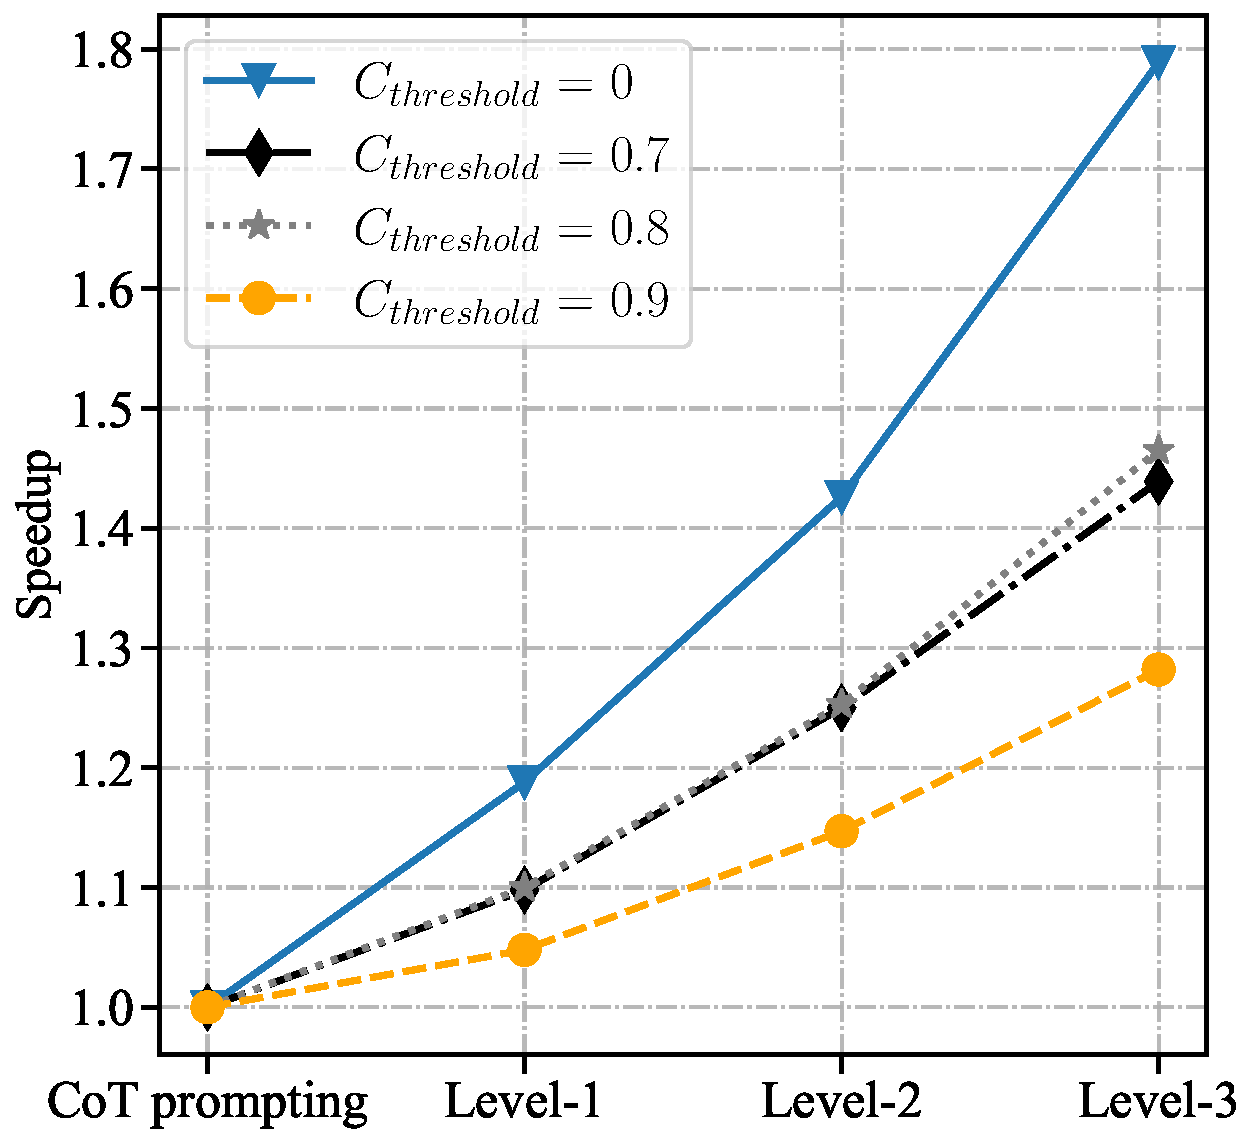
\includegraphics [width =\textwidth]{figures/speedup.pdf}
        \captionsetup{font=small}
        \captionof{figure}{Speedup of inference.}
        \label{fig:speedup}
    \end{minipage}
    % \begin{minipage}{0.22\textwidth}
    %     \centering
    %     \setlength{\abovecaptionskip}{0.1cm}
    %     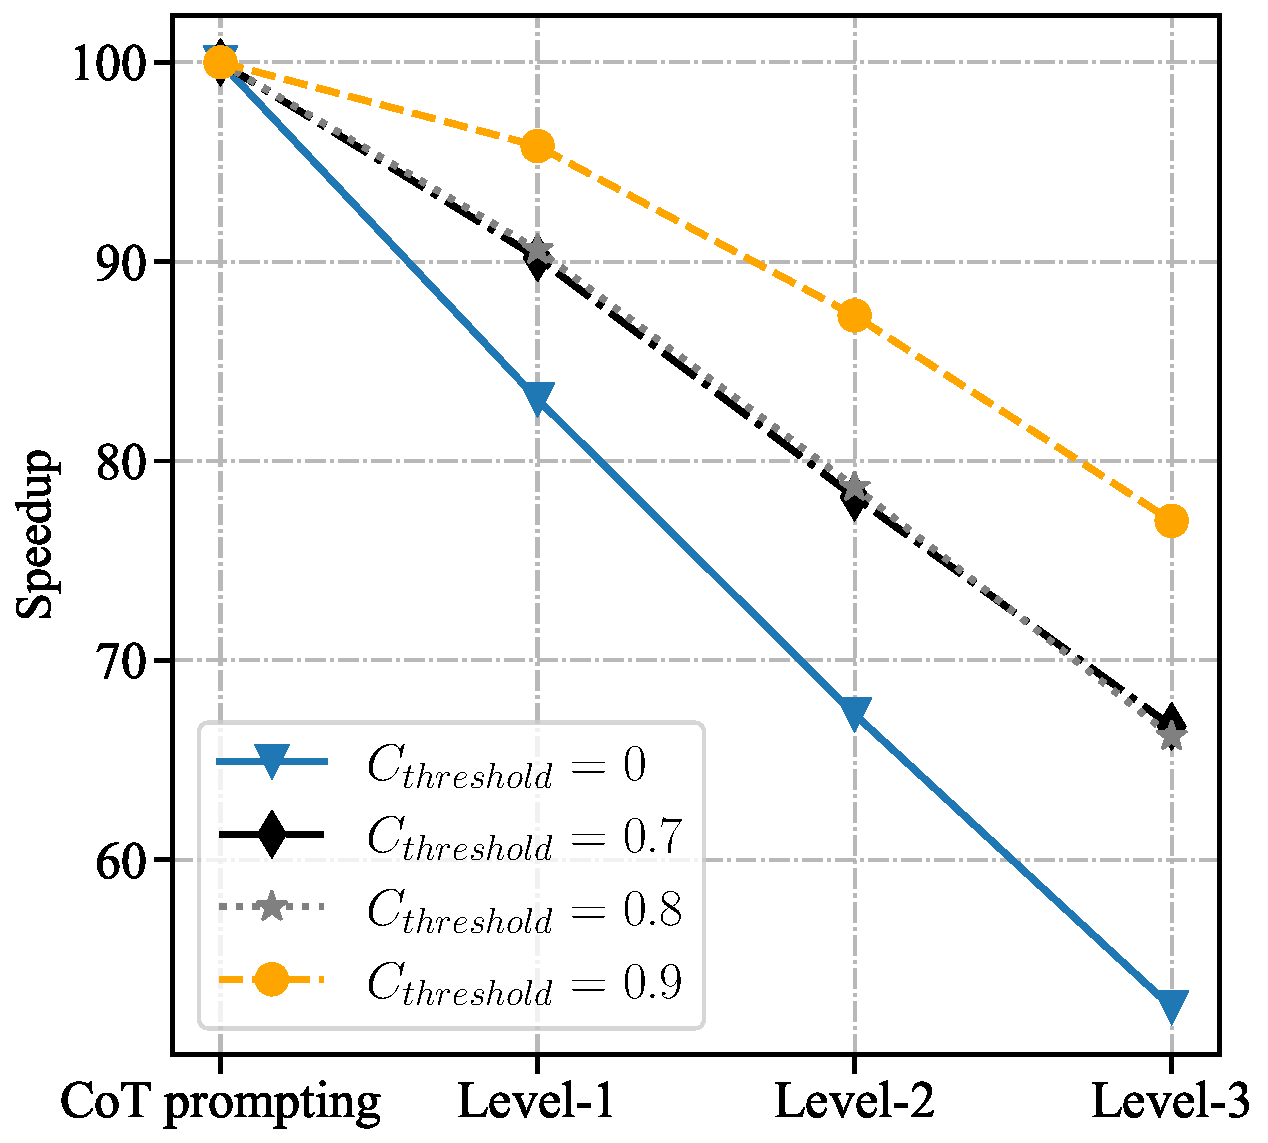
\includegraphics [width =\textwidth]{figures/token.pdf}
    %     \captionsetup{font=small}
    %     \captionof{figure}{Token consumption.}
    %     \label{fig:token}
    % \end{minipage}
    % \vspace{-0.5cm}
\end{figure*}
\vspace{-4mm}
% \begin{table*}[h]
% \centering
% \setlength{\abovecaptionskip}{0.1cm}
% \caption{The evaluation results of path-consistency across various tasks, including (i) Mathematical reasoning: GSM8K, SVAMP, ASDiv, MultiArith (MA); (ii) Commonsense reasoning: StrategyQA (SQA), RuinNames (RN), SalientTranslation (ST); (iii) Symnolic reasoning: BooleanExpression (BE), TrackingShuffledObjects (TSO), LogicalDeduction (LD). $C$=0 indicates that no confidence threshold is applied; the prefix corresponding to the majority element is extracted directly.}
% \label{tab:result}
% \resizebox{\textwidth}{!}{
% \begin{tabular}{@{}cccccccccccccc@{}}
% \toprule
% Dataset&Metrics (\%)&SC&PC \small{($C$=0)}&PC \small{($C$=0.7)}&PC \small{($C$=0.8)}&PC \small{($C$=0.9)}&Dataset&Metrics (\%)&SC&PC \small{($C$=0)}&PC \small{($C$=0.7)}&PC \small{($C$=0.8)}&PC \small{($C$=0.9)} \\
%       \midrule
%       & Acc.     & 64.1 & 66.6 \small{(+2.6)} & 67.1 \small{(+3.1)}  & \textbf{67.8 \small{(+3.8)}} & 66.6 \small{(+2.6)} &    & Acc.     & 76.0 & 71.2 \small{(-4.8)}  & \textbf{74.4 \small{(-1.6)}} & 72 \small{(-4.0)} & 71.6 \small{(-4.4)} \\
% GSM8K & Speedup  & -    & +28.9               & +18.0                & +17.4                        & +10.2               & RN & Speedup  & -    & +10.4                & +7.8                         & +7.4              & +4.7        \\
%       & Decrease & -    & -24.0               & -16.1                & -16.2                        & -9.9                &    & Decrease & -    & -9.8                 & -7.2                         & -6.6              & -4.7        \\ 
%       \cmidrule(lr){2-7} \cmidrule(l){9-14} 
%       & Acc.     & 79.3 & 78.8 \small{(-0.5)} & 78.5 \small{(-0.8)}  & 79.2 \small{(-0.1)} & \textbf{79.9 \small{(+0.6)}} &    & Acc.     & 54.8 & \textbf{58.4 \small{(+3.6)}} & 57.2 \small{(+2.4)} & 56.4 \small{(+1.6)} & 55.2 \small{(+0.4)} \\
% SVAMP & Speedup  & -    & +48.3               & +36.6                & +35.7               & +24.8                        & ST & Speedup  & -    & +30.5                        & +19.6               & +17.3               & +10.2       \\
%       & Decrease & -    & -36.6               & -29.4                & -29.7               & -22.3                        &    & Decrease & -    & -25.8                        & -18.3               & -16.4               & -10.6       \\
%       \cmidrule(l){2-14} 
%       & Acc.     & 81.0 & 80.1 \small{(-0.9)} & \textbf{81.2 \small{(+0.2)}} & 80 \small{(-1.0)}  & 80.6 \small{(-0.4)}   &    & Acc.     & 88.4 & \textbf{90 \small{(+1.6)}}   & 89.6 \small{(+1.2)} & 88.8\small{(+0.4)}  & 89.6 \small{(+1.2)} \\
% ASDiv & Speedup  & -    & +42.0               & +32.1                        & +31.1              & +24.9                 & BE & Speedup  & -    & +26.6                        & +24.3               & +25.2               & +22.0       \\
%       & Decrease & -    & -32.7               & -27.2                        & -27.1              & -22.6                 &    & Decrease & -    & -21.3                        & -19.8               & -20.3               & -18.3       \\
%       \cmidrule(lr){2-7} \cmidrule(l){9-14} 
%       & Acc.     & 96.7 & 97.8 \small{(+1.1)} & 97.2 \small{(+0.5)}  & \textbf{98.9 \small{(+2.2)}} & 98.3 \small{(+1.6)} &    & Acc.     & 54.0 & 58 \small{(+4.0)}  & 56 \small{(+2.0)} & \textbf{59.2 \small{(+5.2)}} & 58.4 \small{(+4.4)}  \\
% MA    & Speedup  & -    & +42.7               & +40.8                & +40.5                        & +33.8               & TSO& Speedup  & -    & +18.4              & +12.9             & +11.3                        & +6.8        \\
%       & Decrease & -    & -34.8               & -33.3                & -33.1                        & -27.2               &    & Decrease & -    & -16.7              & -12.4             & -10.8                        & -6.8        \\
%       \cmidrule(r){1-7} \cmidrule(l){9-14} 
%       & Acc.     & 71.4 & 70.8 \small{(-0.6)} & 70.6 \small{(-0.8)}  & \textbf{71.3 \small{(-0.1)}} & 71.1 \small{(-0.3)} &    & Acc.     & 78.8 & 76.8 \small{(-2,0)} & \textbf{78.8 \small{(+0.0)}} & 77.2 \small{(-1.6)} & 76 \small{(-2.8)}   \\
% SQA   & Speedup  & -    & +34.2               & +29.4                & +24.3                        & +16.4               & LD & Speedup  & -    & +31.6               & +23.1                        & +30.1               & +19.1       \\
%       & Decrease & -    & -27.8               & -24.0                & -22.1                        & -16.0               &    & Decrease & -    & -26.1               & -20.5                        & -24.8               & -17.5       \\
%       \bottomrule
% \end{tabular}
% }
% % \vspace{-0.5cm}
% \end{table*}


\Cref{tab:speedup} presents the performance and efficiency of path-consistency on the GSM8K dataset across different confidence thresholds and prefix levels. The experiments compare path-consistency with the basic self-consistency method in terms of task accuracy, inference latency, and token consumption. 
The results show that path-consistency reduces inference latency across all confidence thresholds, with a maximum speedup of 28.9\%, while maintaining or improving accuracy on GSM8K.
As the prefix level increases, later branches reuse longer prefixes and therefore require fewer newly generated tokens, leading to larger speedups, reaching up to 78.9\% at level-3 while maintaining at least 27.0\%, as shown in \cref{fig:speedup}. 

\subsubsection{Performance on Different Tasks}

\begin{table*}[b]
\centering
\setlength{\abovecaptionskip}{0.1cm}
\caption{The evaluation results of path-consistency across various tasks, including (i) Arithmetic reasoning: GSM8K, SVAMP, ASDiv, MultiArith (MA); (ii) Commonsense reasoning: StrategyQA (SQA), RuinNames (RN), SalientTranslation (ST); (iii) Symbolic reasoning: BooleanExpression (BE), TrackingShuffledObjects (TSO), LogicalDeduction (LD). $C$=0 indicates that no confidence threshold is applied; the prefix corresponding to the majority element is extracted directly.}
\label{tab:result}
\resizebox{\textwidth}{!}{
\begin{tabular}{@{}cccccccccccccc@{}}
\toprule
Dataset&Metrics (\%)&SC&PC \small{($C$=0)}&PC \small{($C$=0.7)}&PC \small{($C$=0.8)}&PC \small{($C$=0.9)}&Dataset&Metrics (\%)&SC&PC \small{($C$=0)}&PC \small{($C$=0.7)}&PC \small{($C$=0.8)}&PC \small{($C$=0.9)} \\
      \midrule
      & Acc.     & 64.1 & 66.6 \small{(+2.6)} & 67.1 \small{(+3.1)}  & \textbf{67.8 \small{(+3.8)}} & 66.6 \small{(+2.6)} &    & Acc.     & 76.0 & 71.2 \small{(-4.8)}  & \textbf{74.4 \small{(-1.6)}} & 72 \small{(-4.0)} & 71.6 \small{(-4.4)} \\
GSM8K & Speedup  & -    & +28.9               & +18.0                & +17.4                        & +10.2               & RN & Speedup  & -    & +10.4                & +7.8                         & +7.4              & +4.7        \\
      & Decrease & -    & -24.0               & -16.1                & -16.2                        & -9.9                &    & Decrease & -    & -9.8                 & -7.2                         & -6.6              & -4.7        \\ 
      \cmidrule(lr){2-7} \cmidrule(l){9-14} 
      & Acc.     & 79.3 & 78.8 \small{(-0.5)} & 78.5 \small{(-0.8)}  & 79.2 \small{(-0.1)} & \textbf{79.9 \small{(+0.6)}} &    & Acc.     & 54.8 & \textbf{58.4 \small{(+3.6)}} & 57.2 \small{(+2.4)} & 56.4 \small{(+1.6)} & 55.2 \small{(+0.4)} \\
SVAMP & Speedup  & -    & +48.3               & +36.6                & +35.7               & +24.8                        & ST & Speedup  & -    & +30.5                        & +19.6               & +17.3               & +10.2       \\
      & Decrease & -    & -36.6               & -29.4                & -29.7               & -22.3                        &    & Decrease & -    & -25.8                        & -18.3               & -16.4               & -10.6       \\
      \cmidrule(l){2-14} 
      & Acc.     & 81.0 & 80.1 \small{(-0.9)} & \textbf{81.2 \small{(+0.2)}} & 80 \small{(-1.0)}  & 80.6 \small{(-0.4)}   &    & Acc.     & 88.4 & \textbf{90 \small{(+1.6)}}   & 89.6 \small{(+1.2)} & 88.8\small{(+0.4)}  & 89.6 \small{(+1.2)} \\
ASDiv & Speedup  & -    & +42.0               & +32.1                        & +31.1              & +24.9                 & BE & Speedup  & -    & +26.6                        & +24.3               & +25.2               & +22.0       \\
      & Decrease & -    & -32.7               & -27.2                        & -27.1              & -22.6                 &    & Decrease & -    & -21.3                        & -19.8               & -20.3               & -18.3       \\
      \cmidrule(lr){2-7} \cmidrule(l){9-14} 
      & Acc.     & 96.7 & 97.8 \small{(+1.1)} & 97.2 \small{(+0.5)}  & \textbf{98.9 \small{(+2.2)}} & 98.3 \small{(+1.6)} &    & Acc.     & 54.0 & 58 \small{(+4.0)}  & 56 \small{(+2.0)} & \textbf{59.2 \small{(+5.2)}} & 58.4 \small{(+4.4)}  \\
MA    & Speedup  & -    & +42.7               & +40.8                & +40.5                        & +33.8               & TSO& Speedup  & -    & +18.4              & +12.9             & +11.3                        & +6.8        \\
      & Decrease & -    & -34.8               & -33.3                & -33.1                        & -27.2               &    & Decrease & -    & -16.7              & -12.4             & -10.8                        & -6.8        \\
      \cmidrule(r){1-7} \cmidrule(l){9-14} 
      & Acc.     & 71.4 & 70.8 \small{(-0.6)} & 70.6 \small{(-0.8)}  & \textbf{71.3 \small{(-0.1)}} & 71.1 \small{(-0.3)} &    & Acc.     & 78.8 & 76.8 \small{(-2,0)} & \textbf{78.8 \small{(+0.0)}} & 77.2 \small{(-1.6)} & 76 \small{(-2.8)}   \\
SQA   & Speedup  & -    & +34.2               & +29.4                & +24.3                        & +16.4               & LD & Speedup  & -    & +31.6               & +23.1                        & +30.1               & +19.1       \\
      & Decrease & -    & -27.8               & -24.0                & -22.1                        & -16.0               &    & Decrease & -    & -26.1               & -20.5                        & -24.8               & -17.5       \\
      \bottomrule
\end{tabular}
}
% \vspace{-0.5cm}
\end{table*}
\textbf{Arithmetic Reasoning:}
% \subsubsection{Arithmetic Reasoning.}
\Cref{tab:result}, rows 1-4, shows the task performance on arithmetic reasoning datasets, along with three additional datasets. Path-consistency maintains accuracy close to self-consistency and in some cases improves it under suitable confidence thresholds. On GSM8K, SVAMP, ASDiv, and MultiArith, accuracy improvements of up to 3.8\%, 0.6\%, 0.2\%, and 2.2\% are observed, respectively. Due to the varying difficulty levels of the datasets for the LLM, the optimal confidence threshold differs for each dataset. For instance, higher or lower confidence thresholds may enhance performance on SVAMP and ASDiv.

The results also highlight the efficiency improvements on arithmetic reasoning datasets. Path-consistency achieves acceleration rates of up to 28.9\%, 48.3\%, 42.0\%, and 42.7\% on GSM8K, SVAMP, ASDiv, and MultiArith, respectively, along with a corresponding decrease in token consumption. These results show that the confidence threshold controls a trade-off between prefix reuse and reliability, allowing path-consistency to reduce latency and token consumption while maintaining comparable accuracy.

\textbf{Commonsense Reasoning:}
% \subsubsection{Commonsense Reasoning.}
\Cref{tab:result}, rows 5-7, reports the performance of path-consistency on commonsense reasoning datasets. In terms of task accuracy, path-consistency slightly underperforms compared to the baseline on the StrategyQA and Ruins Names tasks. This decline becomes smaller under more conservative confidence thresholds. On the Salient Translation task, path-consistency still maintains better task performance compared to the baseline. Regarding acceleration, path-consistency provides up to 34.2\%, 10.4\%, and 30.5\% speed improvements on StrategyQA, Ruins Names, and Salient Translation datasets, respectively.

The efficiency gain on Ruin Names is less pronounced than on other datasets. This is because the Ruins Names task is more difficult, with longer inputs and prompts reduce the fraction of generated reasoning tokens that can be saved by prefix reuse.

\begin{wrapfigure}{r}{0.5\textwidth}
\centering
\vspace{-6mm}
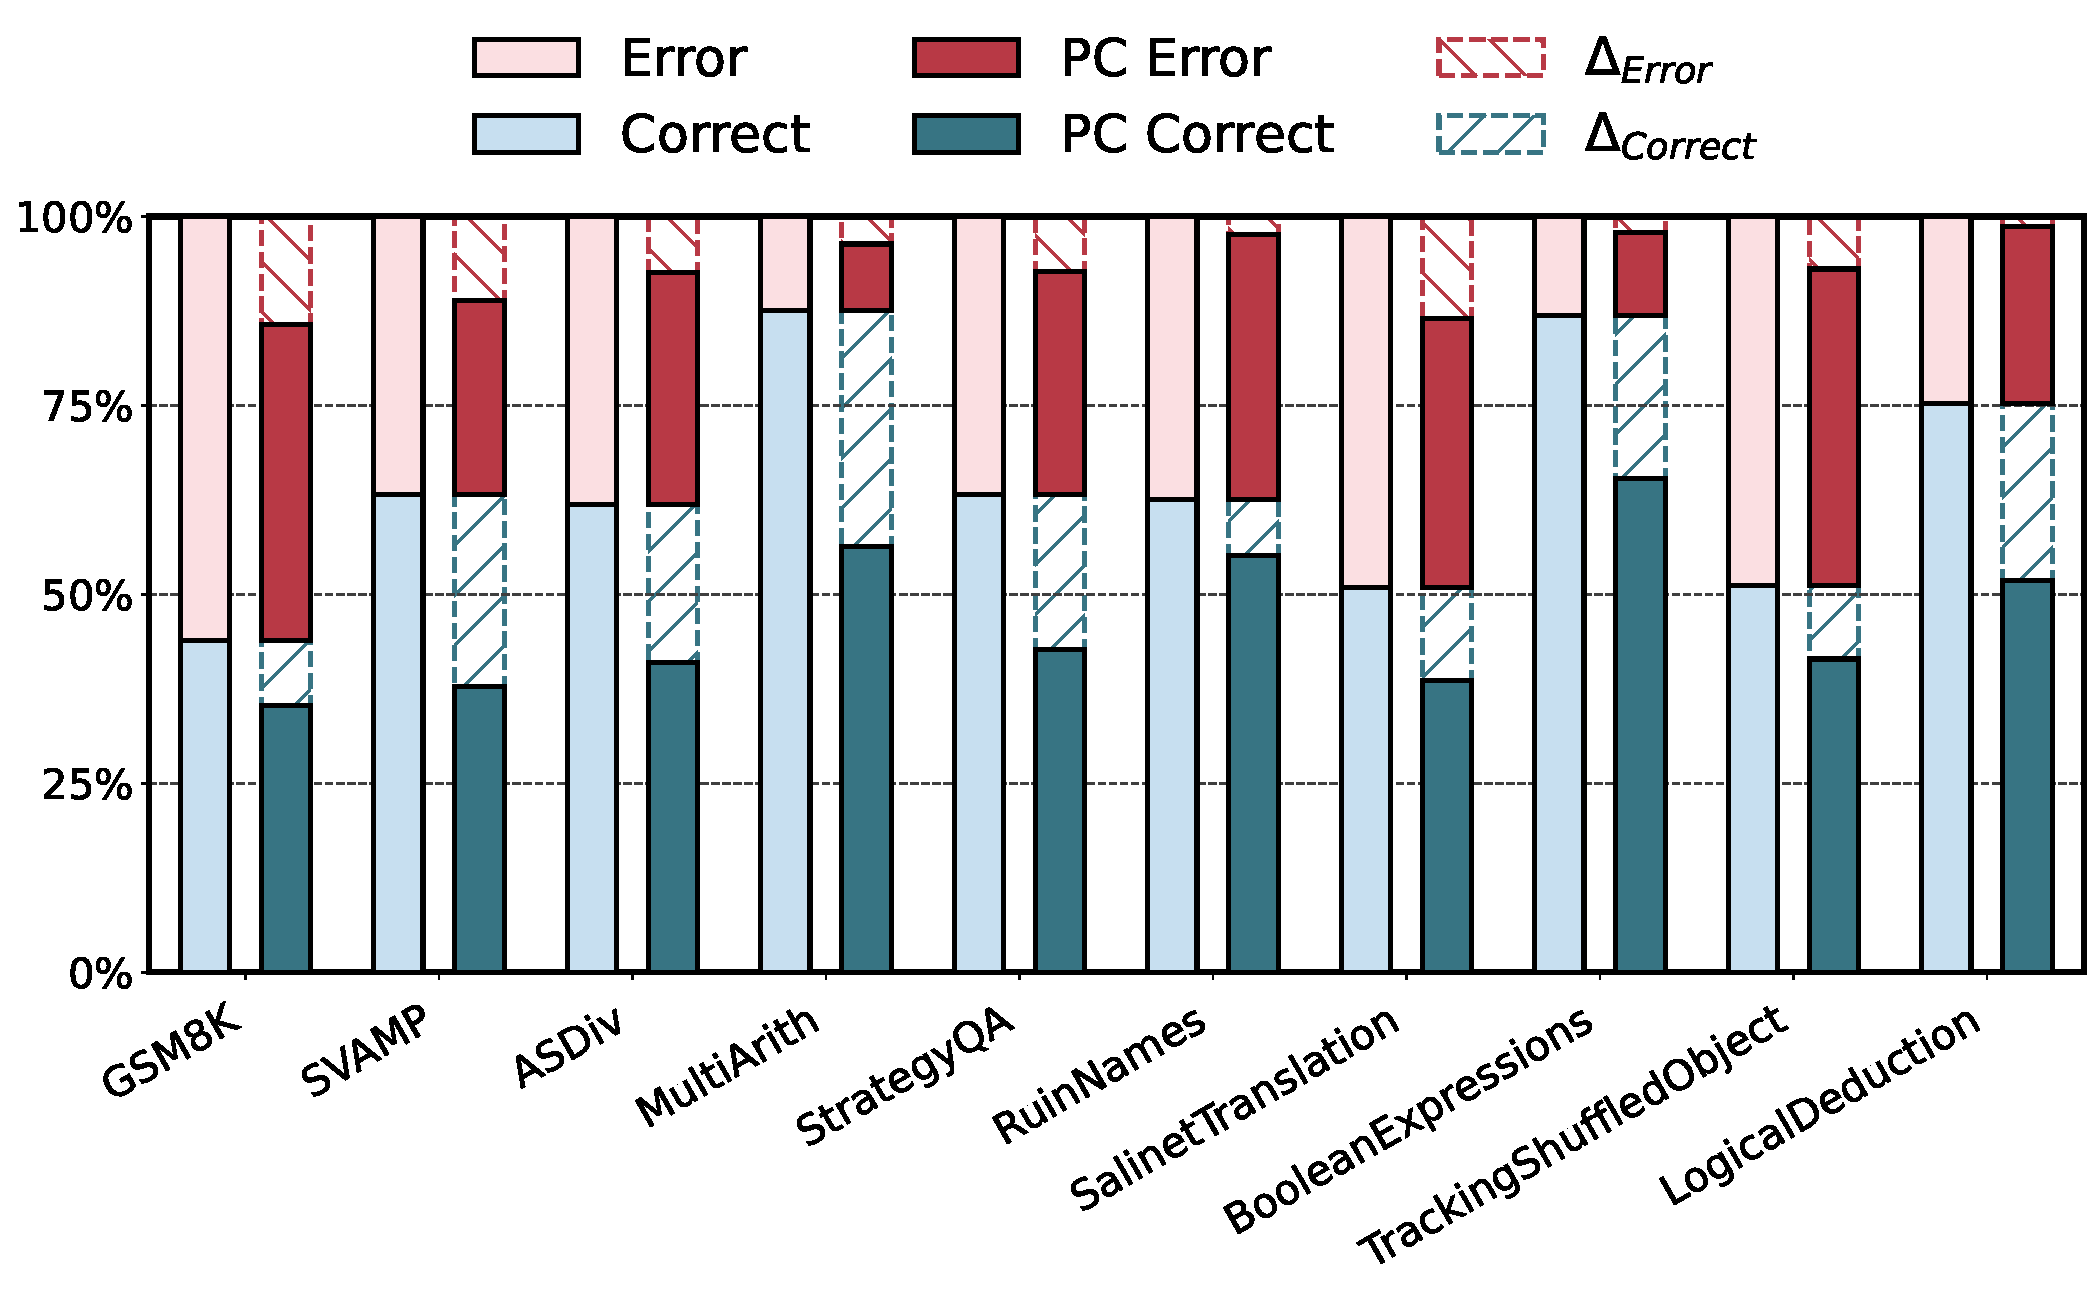
\includegraphics[trim=0cm 0cm 0cm 0cm, clip,height=45mm]{figures/Characterization-chage.pdf}
\vspace{-8mm}
\caption{The change in the proportion of tokens generated by path-consistency on correct or incorrect paths.}
\label{fig:Error and Redundant}
\vspace{-6mm}
\end{wrapfigure}

\textbf{Symbolic Reasoning:}
% \subsubsection{Symbolic Reasoning.}
\Cref{tab:result}, rows 8-10, compares the performance of different methods on the symbolic reasoning datasets. Path-consistency performs exceptionally well in terms of task accuracy, especially in the Tracking Shuffled Objects task, where it achieves the highest improvement of 5.2\% among all datasets. Additionally, compared to the baseline, it delivers approximately a 20\% speedup in inference latency across symbolic reasoning tasks.

In general, lower confidence thresholds indicate a more aggressive prefix selection strategy, often resulting in more significant efficiency improvements. However, in the Logical Deduction task, the efficiency improvement is actually higher at a confidence threshold of 0.8 compared to 0.7. This is because a more aggressive prefix selection strategy is more likely to choose suboptimal prefixes, which makes the subsequent branching generation less effective. Specifically, we found that with a confidence threshold of 0.7, the efficiency improvement at prefix level-2 is more significant than at prefix level-3, as prefix level-3 generates many erroneous paths, leading to this phenomenon.


\subsubsection{Result Analysis}

\begin{wraptable}{r}{0.5\textwidth}
\vspace{-5mm}
  \caption{Impacts of maximum prefix levels of path-consistency on GSM8K.}
  \label{tab:level}
\vspace{-1mm}
\begin{scriptsize}
\setlength{\tabcolsep}{4pt}
    \begin{tabular}{@{}ccccc@{}}
    \toprule
    \multicolumn{1}{l}{Method} & \multicolumn{1}{l}{Level} & \multicolumn{1}{l}{Accuracy (\%)} & \multicolumn{1}{l}{Speedup (\%)} & \multicolumn{1}{l}{Decrease (\%)} \\ \midrule
    PC ($C$=0.7)                       & 3                              & 67.1                        & +18.0                              & -16.1                            \\
                                             & 4                              & 66.3                        & +20.5                              & -20.0                            \\ \midrule
    PC ($C$=0.8)                       & 3                              & 67.8                        & +17.4                              & -16.2                            \\
                                             & 4                              & 67.8                        & +18.0                              & -17.8                            \\ \bottomrule
    \end{tabular}

\end{scriptsize}
\end{wraptable}%

\textbf{Reducing Error and Redundancy:}
In \cref{sec:characterization}, we characterized the challenges of self-consistency. On one hand, it wastes computational resources on incorrect branches. On the other hand, it repeats the same computations without obtaining useful intermediate information. \Cref{fig:Error and Redundant} shows the changes in the proportion of tokens generated by path-consistency on correct or incorrect reasoning paths. The results show a decrease in the number of tokens wasted on incorrect branches. Additionally, for correct branches, there is a significant reduction in redundant tokens, which greatly improves efficiency while maintaining accuracy.

\textbf{Hyperparameters Analysis:}
We explored the impact of prefix extraction frequency on path-consistency. With the setting of 20 branches, if the highest prefix level is set to level-3, the prefix is extracted every 5 branches; if the highest prefix level is level-4, the prefix is extracted every 4 branches. \Cref{tab:level} indicates that maintaining the highest prefix level at level-3 preserves higher task accuracy. Increasing the highest level enables a more aggressive strategy, leading to a more noticeable acceleration.

\subsection{Comparison with Similar Work} 

We compare path-consistency (PC) with three related methods. 
\textit{Self-consistency} (SC)~\cite{wang2022self} is the standard baseline that samples multiple reasoning paths and aggregates final answers through majority voting. 
\textit{Adaptive-consistency} (AC)~\cite{aggarwal2023let} uses confidence-based early stopping, where sampling terminates once a sufficiently confident answer is identified. 
\textit{Early-stopping self-consistency} (ESC)~\cite{liescape} divides sampled branches into equally sized windows and stops when the answers within a window become identical.

As shown in \cref{tab:adapt}, PC achieves accuracy comparable to existing efficient self-consistency methods while consuming fewer tokens. 
AC and ESC reduce test-time cost mainly by terminating the sampling process earlier, which may reduce the diversity benefit of self-consistency under large branching. 
In contrast, PC keeps the multi-path sampling structure and reduces the token cost of later branches by reusing high-confidence prefixes. 
This allows PC to make more efficient use of intermediate reasoning information while preserving the accuracy benefit of self-consistency.

\begin{table*}[t]
\caption{Performance of different efficient self-consistency methods on GSM8K, SVAMP, and StrategyQA. The percentages in parentheses denote token reduction relative to standard self-consistency.}
\label{tab:adapt}
\resizebox{\textwidth}{!}{
\begin{tabular}{@{}lclclcl@{}}
\toprule
       & \multicolumn{2}{c}{GSM8K}              & \multicolumn{2}{c}{SVAMP}              & \multicolumn{2}{c}{StrategyQA}         \\ 
\cmidrule(l){2-3}\cmidrule(l){4-5}\cmidrule(l){6-7} 
Method                      & Accuracy (\%) & Tokens (\# per problem) & Accuracy (\%) & Tokens (\# per problem) & Accuracy (\%) & Tokens (\# per problem) \\ 
\midrule
SC~\cite{wang2022self}      & 68.4          & 3,860                   & 80.4          & 2,321                   & 71.7          & 1,805                   \\
AC~\cite{aggarwal2023let}   & 67.2          & 2,248 (-41.7\%)         & 79.7          & 935 (-59.7\%)           & 71.2          & 706 (-60.9\%)           \\
ESC~\cite{liescape}         & 67.2          & 2,710 (-29.8\%)         & 79.2          & 1,154 (-50.3\%)         & 70.8          & 782 (-56.7\%)           \\
PC                          & 67.8          & 1,630 (-57.8\%)         & 79.2          & 816 (-64.8\%)           & 71.3          & 700 (-61.2\%)           \\ 
\bottomrule
\end{tabular}
}
\end{table*}

\subsection{Discussion on Robustness and Scalability}

Path-consistency does not modify model parameters or the generation objective, making it easy to apply to different autoregressive LLMs. 
To examine whether the prefix reuse mechanism is tied to a specific backbone model, we further evaluate PC on DeepSeek-V3~\cite{liu2024deepseek}. 
As shown in \cref{tab:deepseek}, PC achieves similar accuracy to AC and ESC while consuming fewer tokens across GSM8K, SVAMP, and StrategyQA.

\begin{table*}[h]
\setlength{\abovecaptionskip}{0.1cm}
\caption{Evaluation results of different efficient self-consistency methods on DeepSeek-V3. The percentages in parentheses denote token increase relative to PC.}
\label{tab:deepseek}
\centering
\resizebox{\textwidth}{!}{
\begin{tabular}{@{}lclclcl@{}}
\toprule
       & \multicolumn{2}{c}{GSM8K}              & \multicolumn{2}{c}{SVAMP}              & \multicolumn{2}{c}{StrategyQA}         \\ 
\cmidrule(l){2-3} \cmidrule(l){4-5} \cmidrule(l){6-7}  
Method                      & Accuracy (\%) & Tokens (\# per problem) & Accuracy (\%) & Tokens (\# per problem) & Accuracy (\%) & Tokens (\# per problem) \\ 
\midrule
AC~\cite{aggarwal2023let}   & 91.6          & 828 (+5.34\%)           & 94.7          & 363 (+38.0\%)           & 84.5          & 326 (+41.7\%)           \\
ESC~\cite{liescape}         & 91.6          & 868 (+10.4\%)           & 94.7          & 358 (+36.1\%)           & 84.2          & 315 (+36.9\%)           \\
PC                          & 91.8          & 786                     & 94.7          & 263                     & 84.5          & 230                     \\
\bottomrule
\end{tabular} 
}
\end{table*}

These results suggest that path-consistency is not tied to a specific backbone model. 
Compared with early-stopping based methods, PC consistently reduces token consumption by lowering the cost of later branches rather than only reducing the number of sampled branches. 
Together with the additional experiments on Llama-3.2-1B-Instruct in the Appendix, these results provide evidence that prefix reuse can generalize across different model scales. 
A broader evaluation across more model families and longer reasoning tasks remains future work.


